
%%%%%%%%%%%%%%%%%%%%%%%%%%%%%%%%%%%%%%%%%%%%%%%%%%%%%%%%%%%%%%%%%%%%%%%%%%%%%%%%%%%%%%%
%%%%%%%%%%%%%%%%%%%%%%%%%%%%%%%%%%%%%%%%%%%%%%%%%%%%%%%%%%%%%%%%%%%%%%%%%%%%%%%%%%%%%%%
% 
% This top part of the document is called the 'preamble'.  Modify it with caution!
%
% The real document starts below where it says 'The main document starts here'.

\documentclass[12pt]{article}

\usepackage{amssymb,amsmath,amsthm}
\usepackage[top=1in, bottom=1in, left=1.25in, right=1.25in]{geometry}
\usepackage{fancyhdr}
\usepackage{enumerate}
\usepackage{listings}
\usepackage{graphicx}
\usepackage{float}
\usepackage{multicol}
% Comment the following line to use TeX's default font of Computer Modern.
\usepackage{times,txfonts}
\usepackage{mwe}
\usepackage{caption}
\usepackage{subcaption}





\makeatletter
\renewcommand*\env@matrix[1][*\c@MaxMatrixCols c]{%
  \hskip -\arraycolsep
  \let\@ifnextchar\new@ifnextchar
  \array{#1}}
\makeatother

\newtheoremstyle{homework}% name of the style to be used
  {18pt}% measure of space to leave above the theorem. E.g.: 3pt
  {12pt}% measure of space to leave below the theorem. E.g.: 3pt
  {}% name of font to use in the body of the theorem
  {}% measure of space to indent
  {\bfseries}% name of head font
  {:}% punctuation between head and body
  {2ex}% space after theorem head; " " = normal interword space
  {}% Manually specify head
\theoremstyle{homework} 

% Set up an Exercise environment and a Solution label.
\newtheorem*{exercisecore}{Exercise \@currentlabel}
\newenvironment{exercise}[1]
{\def\@currentlabel{#1}\exercisecore}
{\endexercisecore}

\newcommand{\localhead}[1]{\par\smallskip\noindent\textbf{#1}\nobreak\\}%
\newcommand\solution{\localhead{Solution:}}

%%%%%%%%%%%%%%%%%%%%%%%%%%%%%%%%%%%%%%%%%%%%%%%%%%%%%%%%%%%%%%%%%%%%%%%%
%
% Stuff for getting the name/document date/title across the header
\makeatletter
\RequirePackage{fancyhdr}
\pagestyle{fancy}
\fancyfoot[C]{\ifnum \value{page} > 1\relax\thepage\fi}
\fancyhead[L]{\ifx\@doclabel\@empty\else\@doclabel\fi}
\fancyhead[C]{\ifx\@docdate\@empty\else\@docdate\fi}
\fancyhead[R]{\ifx\@docauthor\@empty\else\@docauthor\fi}
\headheight 15pt

\def\doclabel#1{\gdef\@doclabel{#1}}
\doclabel{Use {\tt\textbackslash doclabel\{MY LABEL\}}.}
\def\docdate#1{\gdef\@docdate{#1}}
\docdate{Use {\tt\textbackslash docdate\{MY DATE\}}.}
\def\docauthor#1{\gdef\@docauthor{#1}}
\docauthor{Use {\tt\textbackslash docauthor\{MY NAME\}}.}
\makeatother

% Shortcuts for blackboard bold number sets (reals, integers, etc.)
\newcommand{\Reals}{\ensuremath{\mathbb R}}
\newcommand{\Nats}{\ensuremath{\mathbb N}}
\newcommand{\Ints}{\ensuremath{\mathbb Z}}
\newcommand{\Rats}{\ensuremath{\mathbb Q}}
\newcommand{\Cplx}{\ensuremath{\mathbb C}}
%% Some equivalents that some people may prefer.
\let\RR\Reals
\let\NN\Nats
\let\II\Ints
\let\CC\Cplx
%%%%%%%%%%%%%%%%%%%%%%%%%%%%%%%%%%%%%%%%%%%%%%%%%%%%%%%%%%%%%%%%%%%%%%%%%%%%%%%%%%%%%%%
%%%%%%%%%%%%%%%%%%%%%%%%%%%%%%%%%%%%%%%%%%%%%%%%%%%%%%%%%%%%%%%%%%%%%%%%%%%%%%%%%%%%%%%
% 
% The main document start here.




%  \textbf{Code:}
%  \begin{center}
%  \lstinputlisting[basicstyle = \footnotesize]{}
%  \end{center}
%  
%  \begin{footnotesize}
%  \begin{verbatim}
%    
%  \end{verbatim}
%  \end{footnotesize}
%  
%  
%  \begin{figure}[H]
%    \begin{center}
%      \caption{}
%    \includegraphics[width = \textwidth]{}
%    \end{center}
%  \end{figure}





% The following commands set up the material that appears in the header.
\doclabel{Stat 605: Homework 7}
\docauthor{Stefano Fochesatto}
\docdate{\today}

\begin{document}

\begin{exercise}{1} Conduct the quadrat test for complete spatial randomness on the cells data set. Carry out the analysis using 
  a 2x2 grid, a 3x3 grid, and a 4x4 grid. Is there evidence of regularity or clustering on one scale but not the others? Use $\alpha = .05$, 
  and carry out just 2-sided test.\\
  Please summarize your results, including a table of counts for each for each of the grid sizes and data sets.\\
  the cell data is included in the spatstat package. 

  \begin{footnotesize}
  \begin{verbatim}
    library(spatstat)
    data(cells)
  \end{verbatim}
  \end{footnotesize}  

  Sample code, which you'll need to modify:

  \begin{footnotesize}
  \begin{verbatim}
    tmp <- quadratcount(cells, nx=2, ny=2 )
    tmp
    plot(tmp)
    quadrat.test(cells, nx=2, ny=2, alternative="two.sided")
  \end{verbatim}
  \end{footnotesize}  
  \solution Let's recall a few ideas behind conducting a formal test for CSR using quadrat data. First note that we obtain counts $y_i$
  for each of the $m$ quadrats, and remember that as a rule of thumb it is suggested that we have $m > 6$ and $y_i > 5$. Our test statistic, the index of dispersion (or $\chi^2$ goodness of fit)
  is computed by,  
  \begin{equation*}
    I = \dfrac{(m-1)s^2}{\bar{y}}. 
  \end{equation*}
  Note that $I$ is approximately distributed by a $\chi^2$ with $(m-1)$ degrees of freedom. Computing the p-values for the various tests we get,
  two-tailed (2x the smaller direction, this was the procedure B statistic which applies distance data. I suppose it is similar for I), 
  \begin{align*}
    H_0&: \text{CSR}\\
    H_a&: \text{Not CSR}\\
  \end{align*}
  right-tailed, 
  \begin{align*}
    H_0&: \text{CSR}\\
    H_a&: \text{Clustered}\\
  \end{align*}
  and left-tailed, 
  \begin{align*}
    H_0&: \text{CSR}\\
    H_a&: \text{Regular}\\
  \end{align*}
  Conducting the two tailed tests in R we get the following counts, p-values, and test statistics, 

  \begin{center}
    \begin{tabular}{c|| c c c}
        grid length & 2 & 3 & 4\\
      \hline 
      p-value        & 0.1518  &  0.3391 & 0.0007283\\
      test statistic & 0.47619 & 4.2857  & 2.9524\\
      count          & 9       &   3     & 2\\
                     & 11      &   6     & 3\\
                     & 12      &   3     & 3\\
                     & 8       &   4     & 2\\
                     &         &   7     & 2\\
                     &         &   6     & 3\\
                     &         &   3     & 4\\
                     &         &   6     & 3\\
                     &         &   4     & 2\\  
                     &         &         & 2\\          
                     &         &         & 2\\          
                     &         &         & 2\\        
                     &         &         & 3\\ 
                     &         &         & 4\\          
                     &         &         & 2\\          
                     &         &         & 3          
     \end{tabular}
    \end{center}
    \textbf{Code:}
    \begin{center}
    \lstinputlisting[basicstyle = \footnotesize]{r1.txt}
    \end{center}

    From the various quadrat tests we find that when using a 4x4 grid we conclude that the on an $\alpha = .05$
    significance level the data does not exhibit complete spatial randomness. This is somewhat expected given the low value of the counts. 
    Considering the ratio between mean and variance for the poisson distribution, with low counts in each quadrant we will find that there is little to no variance across quadrants
    which suggests regularity (performing the one-sided tests corroborates this).
\end{exercise}
\vspace{.5in}

\begin{exercise}{2} Repeat problem 1 for the redwood seedlings / saplings data set. 
  This data set is included in spatstat:
  \begin{footnotesize}
    \begin{verbatim}
      library(spatstat)
      data(redwood)
    \end{verbatim}
    \end{footnotesize}  
    \solution
    Conducting the two tailed tests in R we get the following counts, p-values, and test statistics, 

    \begin{center}
      \begin{tabular}{c|| c c c}
          grid length & 2 & 3 & 4\\
        \hline 
        p-value        &  0.1781 & 0.007333 &  0.0004102\\
        test statistic & 6.5161 & 22.774   & 42.258\\
        count          & 10       &   0       & 0 \\
                       & 17      &   6       & 5 \\
                       & 23      &   13      & 1 \\
                       & 12      &   13      & 9\\
                       &         &   8       & 5 \\
                       &         &   2      & 0 \\
                       &         &   5       & 7 \\
                       &         &   9       & 0\\
                       &         &   6      & 8 \\  
                       &         &          & 3 \\          
                       &         &          & 4 \\          
                       &         &          & 2\\
                       &         &          & 2 \\ 
                       &         &          & 10\\          
                       &         &          & 1 \\          
                       &         &          & 5        
       \end{tabular}
      \end{center}
      \textbf{Code:}
      \begin{center}
      \lstinputlisting[basicstyle = \footnotesize]{r2.txt}
      \end{center}
      Here we can see that with 4 quadrats the csr test concludes that the data exhibit complete spatial randomness, which is questionable given the small number of quadrats. When we consider the 
      9 and 16 csr tests we find that at an $\alpha = .05$ level we get that the data do not exhibit complete spatial randomness. Given the variance (variance is likely larger than the mean) among the counts for 
      the 9 and 16 quadrat csr tests we would likely conclude that the data show significant clustering.  
\end{exercise}
\vspace{.5in}






\begin{exercise}{3} Repeat problem 1 for the black pine seedlings data set.\\
  This data set is posted on Canvas as the file black\_pine\_saplings.txt.\\
  \solution Importing the data, creating a ppp object, then conducting the quadrat test for csr we get the following p-values, test statistics, and counts,


  \begin{center}
    \begin{tabular}{c|| c c c}
        grid length & 2 & 3 & 4\\
      \hline 
      p-value        &  0.6762 & 0.1119   &  0.9028\\
      test statistic &  3.3692 & 15.169   &  15\\
      count          & 22      &  6       & 4\\
                     & 17      &  15      & 8\\
                     & 13      &  7       & 4\\
                     & 13      &  10      & 4\\
                     &         &  4       & 5\\
                     &         &  3       & 5\\
                     &         &  4       & 5\\
                     &         &  8       & 4\\                     
                     &         &  8       & 4\\  
                     &         &          & 1\\          
                     &         &          & 2\\          
                     &         &          & 0\\                     
                     &         &          & 2\\ 
                     &         &          & 6\\          
                     &         &          & 6\\          
                     &         &          & 5\\     
     \end{tabular}
    \end{center}
    \textbf{Code:}
    \begin{center}
    \lstinputlisting[basicstyle = \footnotesize]{r3.txt}
    \end{center}

    With every grid we find that at a $\alpha = .05$ significance level we fail to reject the null hypothesis and conclude that the data exhibit complete spatial randomness. 
    Of the different number of quadrats, I trust the 9 quadrat test the most, since it has more than 6 quadrats with the counts, generally being greater than 5. 
\end{exercise}
\vspace{.5in}





\begin{exercise}{4} Carry out a quadrat test for spatial randomness for each of the three data sets above, using a hexagonal grid with an appropriate grid size. Note the recommendations on page 172
  of the lecture notes. Summarize your results including a table of counts for each data set.\\
  You should exclude partial cells, which means you'll have to do some of the calculations yourself.\\
  Sample code, which you'll need to modify:\\
  \begin{footnotesize}
    \begin{verbatim}
      plot(redwood)
      H <- hextess(redwood, s=2) # s = side length of hexagons
      plot(H)
      plot(quadratcount(redwood, tess=H))
    \end{verbatim}
    \end{footnotesize}
    \solution The following are the hexagonal grid patterns were used to generate the partitions of the data, 


    \begin{figure}[H]
      \centering
      \caption{Hexagonal Partitions}
      \begin{subfigure}[b]{0.45\textwidth}
          \centering
          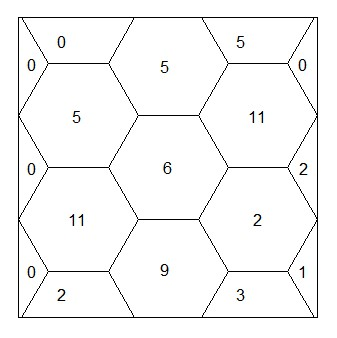
\includegraphics[width=\textwidth]{redwood.jpg}
          \caption{Redwood}
      \end{subfigure}
      \hfill
      \begin{subfigure}[b]{0.45\textwidth}
          \centering
          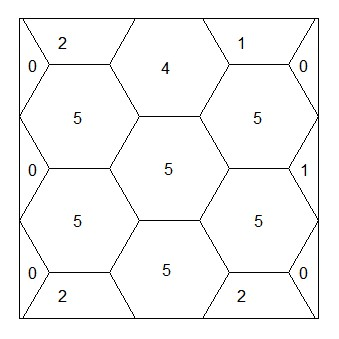
\includegraphics[width=\textwidth]{cells.jpg}
          \caption{Cells}
      \end{subfigure}
      \hfill
      \begin{subfigure}[b]{0.45\textwidth}
          \centering
          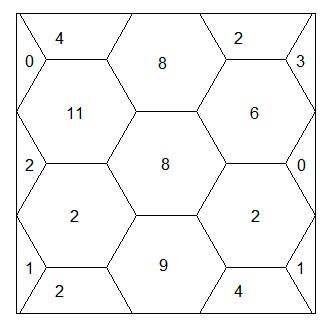
\includegraphics[width=\textwidth]{blackpine.jpg}
          \caption{Blackpine}
      \end{subfigure}
  \end{figure}
  Computing the quadrat test for CSR for each of the full size hexagonal partitions we get the following p-values, test statistics, and counts,
  
  \begin{center}
    \begin{tabular}{c|| c c c}
        Data & Redwood & Cells & Blackpine\\
      \hline 
      p-value        &  0.249304 & 0.0002143529   &  0.1822028\\
      test statistic &  10     & 0.1764706   & 10.91304\\
      count          &  5      &  4          & 11\\
                     &  5      &  5          &  8\\
                     & 11      &  5          &  2\\
                     &  6      &  5          &  8\\
                     & 11      &  5          &  6\\
                     &  9      &  5          &  9\\
                     &  2      &  5          &  2\\                                                                                          
     \end{tabular}
    \end{center}
    \textbf{Code:}
    \begin{center}
    \lstinputlisting[basicstyle = \footnotesize]{r4.r}
    \end{center}

    From the tests we found that the Redwood and Blackpine data failed to reject the null hypothesis at an $\alpha = .05$ significance level and therefore exhibited complete spatial randomness. 
    The tests on the Cells data showed that the at a $\alpha = .05$ significance level the data did not exhibit complete spatial randomness. The one-sided tests on the Cells data showed that 
    the data was regularly spaced. interestingly the Redwood data had a higher p-value than the Blackpine data, even though when plotted the Redwood data looks to be more clustered. 




\end{exercise}

\vspace{.5in}




\begin{exercise}{5} How are the p-values related to the three alternative of the quadrat test, two.sided, regular, and clustered? Answer this question by carrying out test with each of the alternatives 
  for the cells data, using a 3x3 grid. Also, explain what the results of these three tests tell us about the cells data; When we look at  the data, they look regular is this reflected in the test results?
  If not, why not?\\
  \solution As stated before, our test statistic approximates a $\chi^2$ distribution on $n - 1$ degrees of freedom, where $n$ is the number of quadrats. The three alternative quadrat tests come the upper, lower, and two.sided p-values of this 
  null distribution. Carrying out the three alternative tests on the Cells data using a 3x3 grid we get the following summary outputs. \\ 
  \textbf{Code:}
  \begin{center}
  \lstinputlisting[basicstyle = \footnotesize]{r5.txt}
  \end{center}
  Note that the two.sided test produced a p-value of .3391 which is not low enough to reject the null of not exhibiting complete spatial randomness, despite the data looking clearly regular when plotted normally. 
  Considering the two alternative tests for regular and clustered data we found that they got p-values of 0.1695 and 0.8305 respectively. Clearly the test statistic on the $\chi^2$ distribution on 8 degrees of freedom 
  is more towards the left, making the p-value for the regular test smaller, and the p-value for the clustered larger. In any case, the quadrat test is doing a poor job, because the expected counts in each quadrat is lower than 
  what is suggested for performing this test (greater than 5). Looking at the two alternative test we might be able to surmise the the data exhibits more regularity than clustering, but is still not significantly regular to  break from the 
  assumption of complete spatial randomness. Also we can see that to compute the two sided p-value, we double the lower p-value of the other to alternative tests (0.3391 = 2* 0.1695).  

\end{exercise}
\newpage




\textbf{Project Proposal:} For my project I was thinking about mainly working with an existing set of data in the realm of ecological niche modeling. The data that I have to work with uses presence/absence of the Icelandic Rock Ptarmagin as a response, and several 
environmental layers like elevation, temperature, soil quality, and grass cover (as is the case with most habitat modeling endeavour). I have already experimented with making models to predict the RIO (relative index of occurrence, sometimes relative occurrence rate), this work resulted in the creation of the following maps,

  \begin{figure}[H]
    \begin{center}
    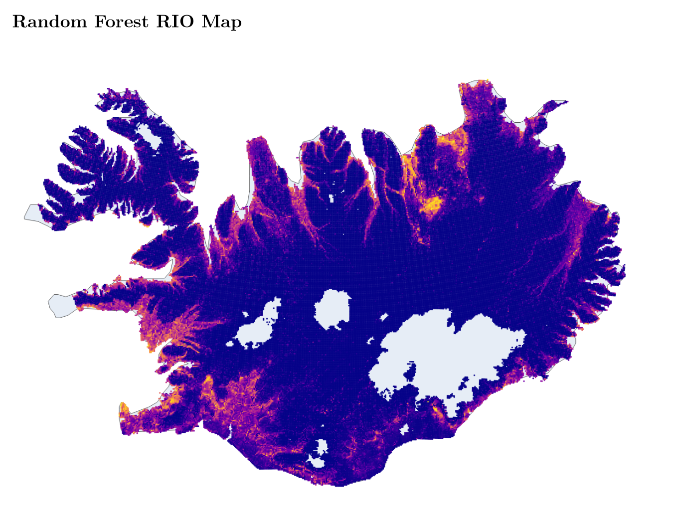
\includegraphics[width = .75\textwidth]{randomforest.png}
    \end{center}
  \end{figure}

  \begin{figure}[H]
    \begin{center}
    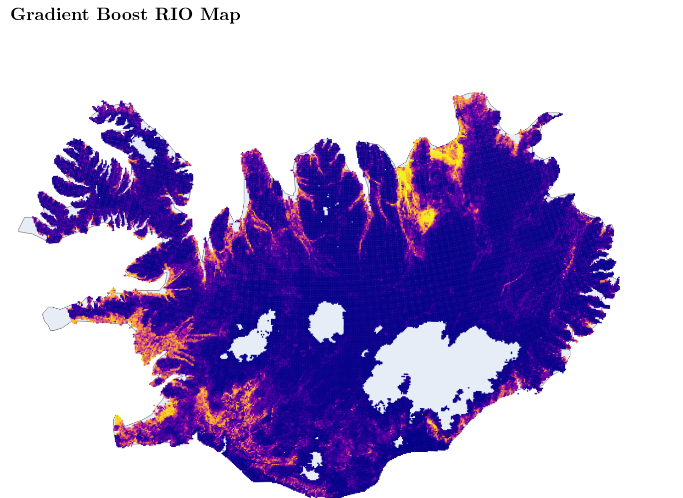
\includegraphics[width = .75\textwidth]{gradientboost.png}
    \end{center}
  \end{figure}

  The main problem that I am hoping to explore is in regard to model validation. The maps were created using Random Forest and Gradient Boosting tree models, for validation 
  I have separate test data in the form of [presence, long, lat], but the rest of my environmental layers are not smoothed maps so using that data to 
  test any model isn't really possible unless we perform some kriging analysis to generate the data at those long, lat pairs. 
  

  










\end{document}


















